\problemname{Slottsmur}

\noindent

Ägaren av slottet Drakfjälls Kastell är rädd för att hans slott ska bli belägrat. Om detta sker vill
han att muren ska vara tålig, så han planerar att förstärka den. Slottsmuren består av $N$ murbitar
som står på en linje. Varje murbit har en viss höjd. Nedan visas ett exempel av hur muren kan se ut.

\begin{center}
  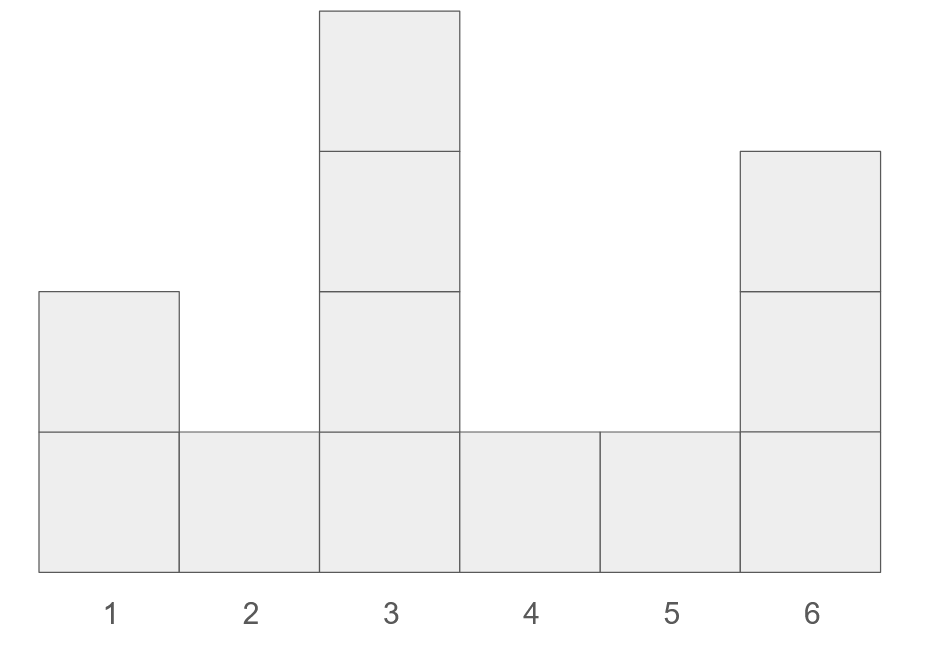
\includegraphics[scale=0.3]{mur1.png}
\end{center}

Slottsägaren är även lite oroad för att hans mur ska drabbas av fuktskador när det regnar, som potentiellt
kan förvärras om han förstärker den. När det
regnar kommer alla murens tomrum att fyllas upp med vatten, så länge vattnet inte kan rinna av
vid sidorna. Om det hade regnat på föregående exempelmur hade vatten samlats vid de blå rutorna.

\begin{center}
  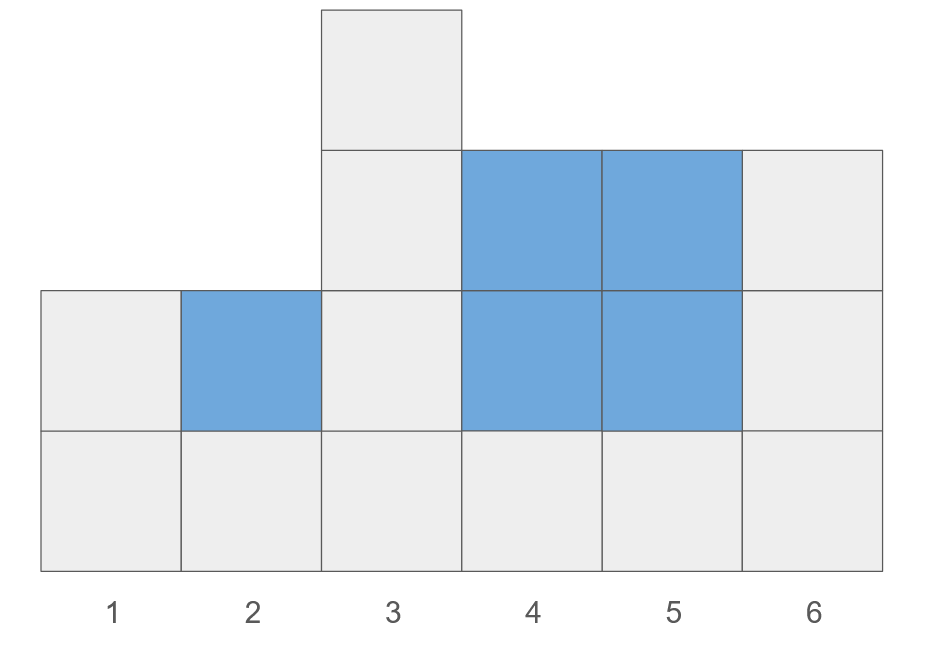
\includegraphics[scale=0.3]{mur2.png}
\end{center}

För att kunna vara strategisk med sin ombyggnad vill han veta hur vissa förstärkningar hade
påverkat mängden regnvatten som samlas i muren om en del av den hade rivts i en belägring.
Till sitt förfogande har han dig, slottets teoretiska datalog.
Slottsägaren kommer att ställa dig två sorters frågor:
\begin{itemize}
  \item Givet är två värden $l$ och $r$. Om alla murbitar rivs förutom de i intervallet 
  $[l,r]$, hur mycket regnvatten hade samlats i muren om det börjar regna?
  Notera att muren inte faktiskt rivs, så detta påverkar inte framtida frågor.
  \item Givet två värden $i$ och $w$, öka höjden på den $i$:te murbiten med $w$. Detta är en
  permanent förändring som kommer att påverka framtida frågor.
\end{itemize}


\section*{Indata}
Den första raden i indatan innehåller heltalen $N$ och $Q$ ($1 \le N, Q \le 2 \cdot 10^5$),
antalet murbitar i muren och antalet frågor.

Därefter följer $N$ heltal $h_1, h_2, \dots, h_N$ ($1 \leq h_i \leq 10^9$), höjden på varje murbit.\\

De följande $Q$ raderna beskriver alla frågor. Varje fråga börjar med heltalet $T$, som antingen är 
$1$ eller $2$.
\begin{itemize}
  \item Om $T=1$ följer $l, r$ ($1 \leq l \leq r \leq N$). Du ska då skriva ut svaret på en fråga av sort $1$ som beskrivet ovan.
  \item Om $T=2$ följer $i, w$ ($1 \leq i \leq N$, $1 \leq w \leq 10^9$). Du ska då öka höjden på den $i$:te murbiten med $w$.
  Det är garanterat att höjden av murbiten förblir mindre än eller lika med $10^9$ efter detta.
\end{itemize}

\section*{Utdata}
För varje fråga av sort $1$, skriv ut mängden vatten som samlas om det börjar regna efter att alla murbitar som ligger utanför
det givna intervallet rivs.

\section*{Poängsättning}
Din lösning kommer att testas på en mängd testfallsgrupper.
För att få poäng för en grupp så måste du klara alla testfall i gruppen.

\noindent
\begin{tabular}{| l | l | p{12cm} |}
  \hline
  \textbf{Grupp} & \textbf{Poäng} & \textbf{Gränser} \\ \hline
  $1$    & $13$       & $N, Q \leq 1000$ \\ \hline
  $2$    & $20$       & Alla frågor är av sort $1$. \\ \hline
  $3$    & $17$       & $h_i$ och $w$ är valda uniformt slumpmässigt bland deras giltiga värden \footnote{Se https://en.wikipedia.org/wiki/Discrete\_uniform\_distribution}. \\ \hline
  $4$    & $23$       & $N, Q \leq 70000$ \\ \hline
  $5$    & $27$       & Inga ytterligare begränsningar. \\ \hline
\end{tabular}

\section*{Förklaring av exempelfall 1}
Vid första frågan ombes vi att beräkna mängden vatten som samlas om vi river allt utanför $[1,6]$. Eftersom
$[1,6]$ utgör hela muren, så rivs inget.
\begin{center}
  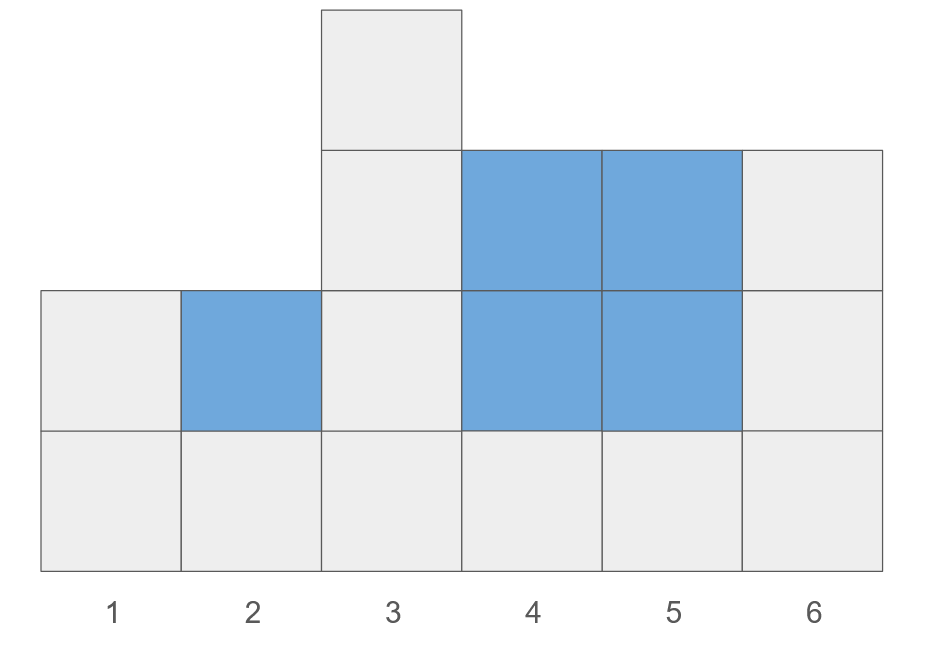
\includegraphics[scale=0.2]{mur2.png}
\end{center}

Vid andra frågan undrar Slottsägaren vad som händer om en del av den högra änden av muren rivits.
De murbitarna som hade rivits markeras med mörgrått. 

\begin{center}
  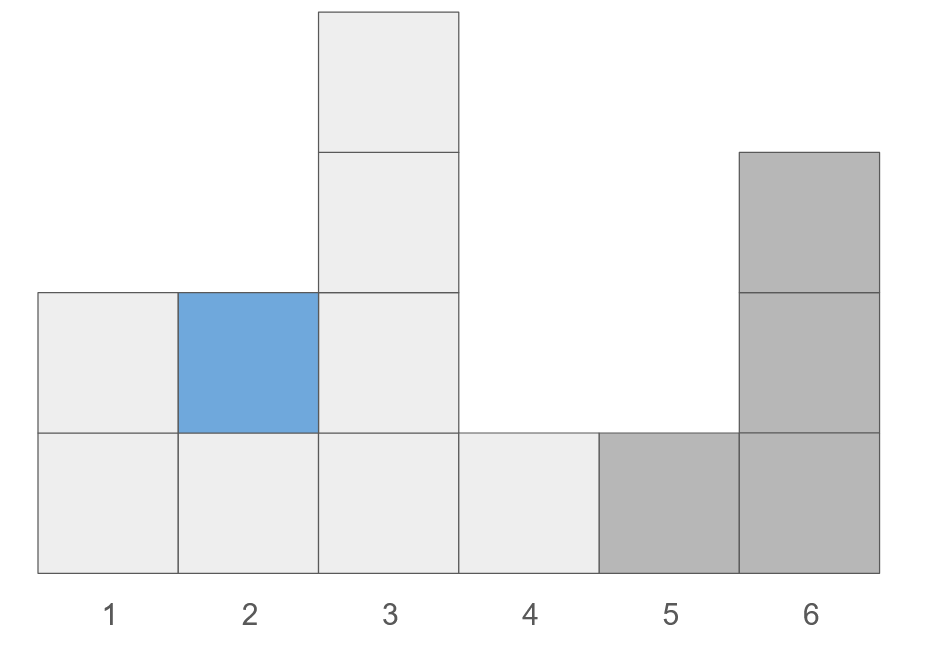
\includegraphics[scale=0.2]{mur3.png}
\end{center}

Vid tredje frågan höjs en del av muren. Detta påverkar den fjärde frågan, som ser ut som följande.

\begin{center}
  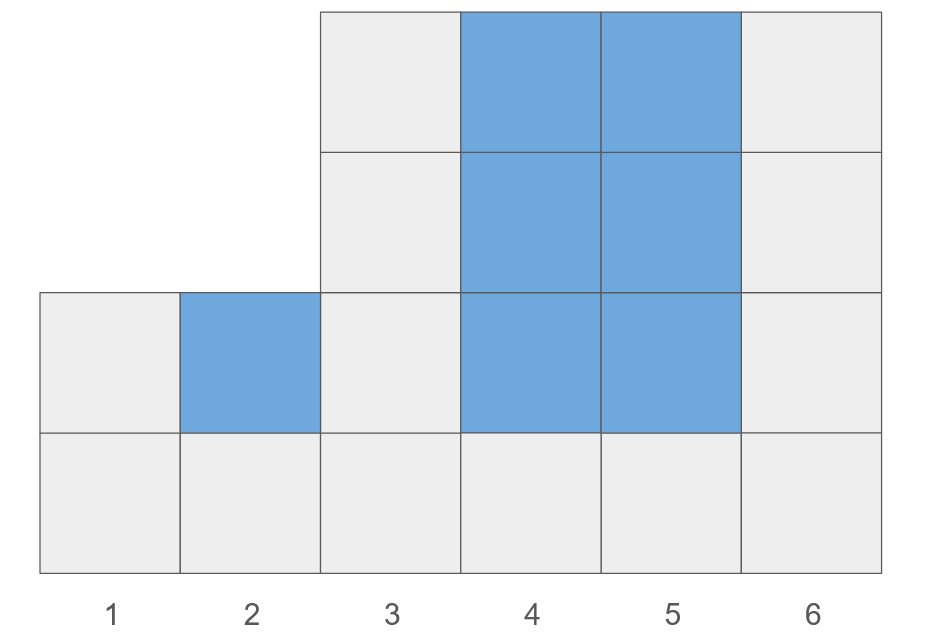
\includegraphics[scale=0.2]{mur4.png}
\end{center}
